% Copyright © 2020-2023 Miguel González Cuadrado <mgcuadrado@gmail.com>

% This file is part of Testudo.

%     Testudo is free software: you can redistribute it and/or modify
%     it under the terms of the GNU General Public License as published by
%     the Free Software Foundation, either version 3 of the License, or
%     (at your option) any later version.

%     Testudo is distributed in the hope that it will be useful,
%     but WITHOUT ANY WARRANTY; without even the implied warranty of
%     MERCHANTABILITY or FITNESS FOR A PARTICULAR PURPOSE.  See the
%     GNU General Public License for more details.

%     You should have received a copy of the GNU General Public License
%     along with Testudo.  If not, see <http://www.gnu.org/licenses/>.

\documentclass[twoside, a4paper, article]{memoir}
%\documentclass[oneside, 11pt, a5paper, article]{memoir}

\usepackage[spanish, british]{babel}
\usepackage[utf8]{inputenc}
\usepackage[T1]{fontenc}
\usepackage{amsmath, amssymb, graphicx, wasysym, bm, fancyvrb, soul, pdfpages}
\usepackage[final]{listings}
\usepackage{tikz, tikzpeople, pgfornament}
\usetikzlibrary{automata, shapes.symbols, patterns}

\newcommand*\testudocolor{\color{red!80!blue}}
\newcommand*\testudo[1]{\texttt{\testudocolor{}#1}}
\newcommand*\testudopair[2]{\testudo{#1}~--~\testudo{#2}}
\newcommand*\keywordcolor{\color{blue!80!red}}
\sethlcolor{red}

\newcommand\chaptertestudopair[3]{%
  \chapter[#1]{#1: \testudopair{#2}{#3}}}
\newcommand\sectiontestudopair[3]{%
  \section[#1]{#1: \testudopair{#2}{#3}}}
\newcommand\subsectiontestudopair[3]{%
  \subsection[#1]{#1: \testudopair{#2}{#3}}}
\newcommand\subsubsectiontestudopair[3]{%
  \subsubsection[#1]{#1: \testudopair{#2}{#3}}}

\newcommand*\ok[1]{\textcolor{green}{#1}}
\newcommand*\fail[1]{\textcolor{red}{#1}}
\newcommand*\blue[1]{\textcolor{blue}{#1}}
\newcommand*\lines[1]{\textcolor{orange}{#1}}
\newcommand*\openbrace{\{}
\newcommand*\closebrace{\}}
\newcommand*\atsign{@}

\newcommand*{\cpplistingindent}{1.25em}
\input{keywords.tex}

\newcommand\typesetexample[1]{%
  \typesetexamplesource{#1}
}

\newcommand\typesetexampleandreport[1]{%
  \typesetexamplesource{#1}
  \typesetexamplereport{#1}
}

\providecommand\typesetexamplereport[1]{%
  \input{reports/#1-cl}%
  \input{reports/#1-op}%
}
\providecommand\typesetexamplesource[1]{%
  \input{examples/#1-lc-cl}%
  \input{examples/#1-uc-op}%
}

\providecommand*\styletext{%
  first in the ``\texttt{lc}'', more cluttered style, then in the
  ``\texttt{uc}'', more open style}

\providecommand*\openingbracesstyletext{%
  Incidentally, in the ``\texttt{lc}''-style examples, opening braces don't
  start a new line, whereas in the ``\texttt{uc}''-style examples they are
  written on their own line.  This has nothing to do with the style, and you
  can write opening braces however you want.}

\newcommand*\commonlistinglstset{%
  \lstset{numbers=left,numberstyle=\tiny, stepnumber=1, numbersep=1em,
    xleftmargin=\cpplistingindent,
    lineskip=0.05pt, % this closes a gap that appears above the line whenever
                     % there are brackets in a comment
    columns=fullflexible,
    basicstyle=\ttfamily,
    keywordstyle=\ttfamily\bfseries,
    emphstyle=\ttfamily\testudocolor{},
    commentstyle=\rmfamily\itshape,
    resetmargins=true,
    backgroundcolor=\color{black!5},
    showstringspaces=false, keepspaces=true, texcl=true, escapechar=|,
    extendedchars=true, literate=%
    {ú}{{\'u}}1%
  }%
}
\newcommand*\cpplistinglstset{%
  \commonlistinglstset{}%
  \lstset{language=[testudo]C++}%
}
\lstnewenvironment{cpplisting}[1][]{%
  \cpplistinglstset{}%
  \lstset{#1}}{}

\newcommand*\bashlistinglstset{%
  \commonlistinglstset{}%
  \lstset{language=bash,
    backgroundcolor=\color{blue!5},
  }%
}
\lstnewenvironment{bashlisting}[1][]{%
  \bashlistinglstset{}%
  \lstset{#1}}{}

\newcommand*\makelistinglstset{%
  \commonlistinglstset{}%
  \lstset{language=make,
    backgroundcolor=\color{red!5},
  }%
}
\lstnewenvironment{makelisting}[1][]{%
  \makelistinglstset{}%
  \lstset{#1}}{}

\usepackage{microtype}
%% \usepackage[textosf, mathlf, italicgreek, openg, footnotefigures%, opticals
%% ]%
%% {MinionPro} % no minionint since it fails
\usepackage{lmodern} % for the bold tt
\usepackage[oldstyle, altP, sups]{fbb}

\usepackage[pdfborder={0 0 0}]{hyperref}

%\setlrmarginsandblock{1cm}{1cm}{*}
%\setulmarginsandblock{2cm}{2cm}{*}
%\checkandfixthelayout

\newcommand*\ellipsis{\,\ldots}
\newcommand*\Cpp{C\texttt{++}}

\firmlists

\newcommand*\indentitem{\hspace*{1em}}

\providecommand*\styleedition{%
  ``\texttt{lc}''- and ``\texttt{uc}''-style edition}

\title{\protect\includegraphics[width=\textwidth]%
  {ascii_logo_colour_cropped.pdf}\\%[1em]%
  Testudo,\\an automatic test system\\for \Cpp{} code\\[1em]%
  \styleedition{}\\[1em](version \protect\input{version}\unskip)}

\author{Miguel González Cuadrado\\\textsf{<mgcuadrado@gmail.com>}}

\maxsecnumdepth{subsection}
\maxtocdepth{subsection}

\begin{document}

% from titlepages.tex
\newlength{\tpheight}\setlength{\tpheight}{0.9\textheight}
\newlength{\txtheight}\setlength{\txtheight}{.9\tpheight}
\newlength{\tpwidth}\setlength{\tpwidth}{0.9\textwidth}
\newlength{\txtwidth}\setlength{\txtwidth}{0.9\tpwidth}
\newlength{\drop}
\newcommand*{\titleGM}{\begingroup% Gentle Madness
\drop = 0\txtheight
\vspace*{\baselineskip}
\vfill
  \hbox{%
  \hspace*{0.2\txtwidth}%
  \rule{1pt}{.9\txtheight}
  \hspace*{0.05\txtwidth}%
%\fbox{%
\parbox[b]{0.75\txtwidth}{
  \vbox{%
    \vspace{\drop}
    \hspace*{-.1\textwidth}%
    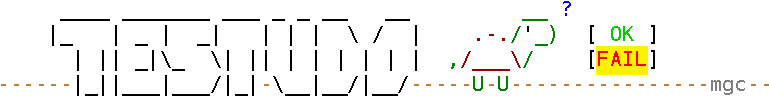
\includegraphics[width=\textwidth]{ascii_logo_colour_cropped.pdf}\\[1em]
    {\HUGE\bfseries Testudo}\\[2\baselineskip]
    {\Large\itshape An automatic test system\\[.2\baselineskip]for
      \Cpp{} code}\\[.5\baselineskip]
    {\hspace*{.05\txtwidth}\Large\itshape
      \protect\styleedition}\\[.5\baselineskip]
    {\hspace*{.05\txtwidth}\Large\itshape
      version \protect\input{version}}\\[3\baselineskip]
    {\Large
      Miguel González Cuadrado\\[.5\baselineskip]<mgcuadrado@gmail.com>}\par
    \vspace{0.47\txtheight}
    {\noindent
      % \hspace{-.5em}\raisebox{-1em}{\includegraphics[height=5em]{chc-cropped}}%
      \hspace{-.3em}The $\chi$ Press}\\[\baselineskip]
    }% end of vbox
}% end of parbox
%}% end of fbox
  }% end of hbox
\vfill
\null
\endgroup}

\titleGM

\thispagestyle{empty}

\clearpage

\vspace*{\fill}
% \hspace{-.5em}\raisebox{-1em}{\includegraphics[height=5em]{chcs}}%
% \hspace{-.3em}The $\chi$ Press

\vspace{.2\textheight}
\begin{small}
\input{copyright.txt}
\end{small}

\thispagestyle{empty}

\cleardoublepage

\frontmatter

\maketitle

\tableofcontents*
\listoffigures*
\listoftables*

\cleartooddpage

\begin{quote}
  \emph{This manual is in its early stages.  I'm going first for completeness,
    not for clarity.  My plans: finish covering the functionality of Testudo,
    convert into a web-friendly format, turn it into a guide rather than a
    dense reference.}
\end{quote}

\chapter{Intro}
\label{cha:intro}

Automatic testing: unit testing, integrated testing, test-driven
development\ellipsis{}  You can do all of these with Testudo.

Brief rundown of Testudo's features:
\begin{itemize}
\item tree-like organisation of tests (\Sref{cha:tests-test-hierarchies});
\item execution of selected tests;
\item easy definition of tests (\Sref{cha:test-steps});
\item clear, complete, flexible test reports;
\item straightforward syntax for declarations, actions, showing values, checks
  on values, and scopes (\Sref{cha:test-steps});
\item support for exception checks (\Sref{sec:exception-checks}) and unexpected
  exceptions (\Sref{sec:unexpected-exceptions-crashes});
\item support for complex types (\Sref{cha:testudo-support-stl-types});
\item easy support for new types (\Sref{cha:adding-testudo-support-your-types});
\item fixtures (\Sref{cha:fixtures});
\item repeating steps for many values, like theorem checking
  (\Sref{cha:with-data-loops});
\item mock objects (\Sref{cha:mock-objects}).
\end{itemize}

\vspace{1\baselineskip}

\begin{quote}
  \emph{``Testudo'' means ``turtle'' in Esperanto and Latin.  The name of the
    turtle in the logo (see the title of this document) is Testarudo, which
    means ``stubborn'' in Spanish.  Testarudo is indefatigable, and will
    tenaciously flag you errors, until you correct them.}
\end{quote}

\vspace{1\baselineskip}

Testudo runs a suite of tests specified by the user, and produces an
\textsc{xml} printout of the results.  You can convert the \textsc{xml} file
into a variety of formats, for immediate perusal, result tracking, statistics,
publication, et cetera.  The blue question mark and the green \verb|[ OK ]| and
red \verb|[FAIL]| flags in the logo are a reference to the way instructions,
passes, and fails are displayed when a test result is converted to a text
report with colours\footnote{Colour-blind-friendly, by the way.}.

A \emph{test suite} in Testudo is composed of an ordered series of
\emph{tests}, each test consisting of a sequence of \emph{steps}.  Tests are
organised as a tree, with test nodes, and proper tests on some test nodes.

When a test suite is run, all tests are performed in order, according to their
position in the test tree, and within each test, the test steps are executed in
order.  Some test steps are \emph{checks}, which can succeed or fail.  Check
successes and failures are tallied and summarised at the end of their test.
Accumulated tallies are also kept for each test node, which combine the tallies
of the sub-tree rooted at each test node.

\section{Macros}
\label{sec:macros}

Testudo relies rather heavily on code generation with \Cpp{} macros.  As
explained in~\Sref{cha:test-output-formats}, you can customise the names of all
the macros to suit your needs or preferences.  In the examples given in this
documents, macros are highlighted like this (here, the macro is
``\texttt{PERFORM}''):
\begin{cpplisting}
PERFORM(firefly.say("Then, it's war!"));
\end{cpplisting}

Testudo macros are coded in such a way that they are impervious to the common
problem of macro arguments containing commas, like for instance in templated
types, which would normally confuse \Cpp{} macros (an argument such as
``\texttt{map<int, float>}'' would be parsed as two arguments:
``\texttt{map<int}'' and ``\texttt{float>}'').  Testudo achieves this by one of
two means:
\begin{itemize}
\item having a single potentially macro-fooling argument for a macro, and
  having it be the last one;
\item requiring parentheses around potentially macro-fooling arguments (this
  will always be made clear in this document).
\end{itemize}

\section{The \texttt{testudo} namespace}
\label{sec:testudo-namespace}

All (non-macro) names defined by Testudo that are intended for usage by users
are defined in the ``\texttt{testudo}'' namespace.  This namespace will left
out in the examples, as if ``\texttt{using namespace testudo}'' had been
declared.

\section{Showcase: code, test, and report}
\label{sec:showcase}

As a quick, self-paced introduction to Testudo test step syntax, i've laid out
hereafter the source code for a class, the source code for a test for the
functionality, and the resulting test report.  If my \LaTeX{} trickery doesn't
fail me, and you have printed this on physical paper, you'll have the source
code for the test and the test report on opposite pages
(pages~\pageref{pag:example-test-code} and~\pageref{pag:example-test-report}),
so you can't better understand how one relates to the other.

The code is meant for this showcase, not for production, and shouldn't be
construed as an example of good coding: you'll see questionably design and
coding practices; you'll see bugs and unimplemented functionality so they can
be pointed out in the report as test fails; you'll see weird vertical spacing
to achieve syncing between the two printed pages; and you'll see too many
concerns crammed into a single test.

In the report, you'll see different colours for different elements:
\begin{itemize}
\item \lines{orange} is for separation, test header cartouches, and line number
  info; in test headers, the full file and line number info is given; for
  individual steps, only the line number is given, unless the step isn't in the
  same file as the test header it's a part of, in which case the full file and
  line number info is written;
\item step type codes, test punctuation, and test summaries are written in
  \blue{blue};
\item \textsc{ok}, fail, and error tags have their own, obvious colour schemes;
\item \fail{red} strings of dashes make it easy to match non-\textsc{ok} tags
  to their steps.
\end{itemize}

\cleartooddpage

{%
  \cpplistinglstset{}%
  \lstinputlisting[language={[testudo]C++}]{testudo_doc.ttd}
}

\newpage

\label{pag:example-test-report}

\input{reports/testudo.use_instructions.tex}

\section{Development workflow with Testudo}
\label{sec:development-workflow-with-testudo}

Testudo can be used with any workflow, with any testing philosophy.  You can
use~it
\begin{itemize}
\item for test-driven development;
\item to translate requirements into tests;
\item to validate specifications;
\item to continuously refactor code;
\item to successfully refactor \emph{legacy} code;
\item to avoid reappearing bugs by turning them into tests;
\item to simply ensure your code is as bug-free as possible.
\end{itemize}

This is how you can use Testudo to improve your development workflow:
\begin{itemize}
\item code Testudo tests for your code, either before the code itself (as in
  \textsc{tdd} and extreme programming), at the same time as the code, or after
  the code (for refactoring, for instance);
\item use Testudo to run the tests often; integrate test running into your
  development cycle and discipline; for instance, you can institute a rule that
  every commit must leave the code with no failed checks or errors; or, if you
  have turned your requirements into tests, your rule can be about never
  introducing regressions;
\item use Testudo to check the progress of your development, by committing the
  report status with every code commit; thus, you can know what the test result
  changes are for your working directory compared to the last committed
  revision, or compare any two revisions.
\end{itemize}

\begin{figure}
  \centering
  \begin{tikzpicture}[
      x=2.5em, y=2em,
      rounded corners,
      every node/.append style={text depth=0.4ex, text height=1.4ex},
      big node/.style={text depth=, text height=},
      no rounded/.style={rounded corners=0},
      printout/.style={
        draw, big node, no rounded, tape, tape bend top=none,
        minimum width=5em, minimum height=3em,
        fill opacity=.5, pattern=horizontal lines light gray,
        text opacity=1}]
    \node[no rounded, pilot, monitor, minimum size=3em] (programmer)
      at (-1, -1.2) {};
    \node[big node] (write edit) at (0,0)
      {\itshape\begin{tabular}{@{}c@{}}write\\\& edit\end{tabular}};
    \node (code) at (3, 1) {\bfseries code};
    \node (tests) at (3, -1)
      {\bfseries\begin{tabular}{@{}c@{}}test\\code\end{tabular}};
    \node (track) at (3, -3) {\bfseries track};
    \draw[->] (write edit) -- +(1.5, 0) |- (code);
    \draw[->] (write edit) -- +(1.5, 0) |- (tests);
    \node(binaries) at (7, 1) {binaries};
    \draw[->] (code) -- node[above, pos=.6]{\itshape build} (binaries);
    \node[draw, big node] (run) at (7,-1)
      {\begin{tabular}{c}Testudo\\``\texttt{run}''\end{tabular}};
    \draw[->] (binaries) -> (run);
    \draw[->] (tests) -> (run);
    \draw[->] (run) |-
      node[big node, below left]
        {\itshape\begin{tabular}{r@{\,\,}}current\\track\end{tabular}}
      (track);
    \node[draw, big node] (diff) at (7,-6)
      {\begin{tabular}{c}Testudo\\``\texttt{diff}''\end{tabular}};
    \draw[->] (run) -- (diff);
    \node[draw, big node] (version) at (3, -6)
      {\begin{tabular}{c}version\\control\end{tabular}};
    \draw[->] (version) --
      node[below=2ex]{\itshape\begin{tabular}{c}versioned\\tracks\end{tabular}}
      (diff);
    \draw[no rounded=0, fill=gray, opacity=.2]
      (version.north) -- (4.5, -3.75)
      -- (4, -3.75) -- (4, 2) -- (2, 2) -- (2, -3.75)
      -- (1.5, -3.75)
      -- node[opacity=1, below, pos=.22]{%
        \itshape\begin{tabular}{r}simultaneous\\commit\end{tabular}} cycle;
    \node[printout] (report) at (10, -1)
      {\itshape\begin{tabular}{@{}c@{}}test\\report\end{tabular}};
    \node[printout] (progress) at (11.5, -6)
      {\itshape\begin{tabular}{@{}c@{}}progress\\tracking\end{tabular}};
    \draw[->] (run) -- (report);
    \draw[->] (diff) -- (progress);
    \coordinate (above write edit) at (3, 3);
    \draw (report) |- (above write edit);
    \draw[->] (progress) |- (above write edit)
      -| ($(programmer.north)+(0,.4)$);
  \end{tikzpicture}
  \caption{Development workflow with Testudo}
  \label{fig:workflow}
\end{figure}

\fref{fig:workflow} shows how Testudo is integrated into a workflow:
\begin{itemize}
\item you write and edit code, and tests for your code;
\item you build your binaries using your build system;
\item you use Testudo to run the tests on your binaries;
\item based on the test reports you get, you make changes to your code and
  tests to ensure quality;
\item Testudo also generates \emph{tracks}; tracks are files that Testudo uses
  to track the test result progress between different versions of your code;
\item when you're happy with your code and changes, you commit them; it's
  important that you commit your code, your tests, and your test tracks
  \emph{simultaneously}; they act as a single, coherent entity;
\item at any moment, you can use Testudo to report the difference between two
  tracks; the difference can be between the latest committed track and your
  current track (``how am i doing with this change?''), or between two
  committed tracks (``what was the progress between these two versions?''); the
  progress tracking also informs your changes to your code and tests.
\end{itemize}

\cleartoevenpage

\addcontentsline{toc}{chapter}{The race}

\newlength\pdfpagehoroffset
\setlength\pdfpagehoroffset{\spinemargin}
\addtolength\pdfpagehoroffset{.5\textwidth}
\addtolength\pdfpagehoroffset{-.5\paperwidth}

\includepdf[pages=-, pagecommand={}, offset=\pdfpagehoroffset{} 0mm]{the_race}


\mainmatter


\chapter{Installation}

In the ``\texttt{testudo}'' directory, do
\begin{itemize}
\item install Testudo with
\begin{bashlisting}
make install
\end{bashlisting}
\item uninstall Testudo (asking confirmation for each deletion) with
\begin{bashlisting}
make uninstall
\end{bashlisting}
\item check installation parameters with
\begin{bashlisting}
make cat_install_params
\end{bashlisting}
\end{itemize}

By default, Testudo installs itself to ``\texttt{\$HOME/local}'', where
``\texttt{\$HOME}'' is the user's home directory.  You can change this by
defining an environment variable ``\texttt{PREFIX}", or by passing
``\texttt{make}'' such a variable.  The following commands are equivalent, and
they will both install Testudo to ``\texttt{/usr/local}'':
\begin{itemize}
\item \texttt{PREFIX=/usr/local make install}
\item \texttt{make PREFIX=/usr/local install}
\end{itemize}


\chapter{Test output formats}
\label{cha:test-output-formats}

When a test suite is run, Testudo outputs a printout detailing each test node,
test, test step, and tallies.  There are several formats for the printout.  You
must choose the format by passing to the executable the flag ``\texttt{-f}''
followed by the name of the format.  Standard formats are ``\texttt{xml}'' and
``\texttt{color\_text}'', but you can add your own.

The ``\texttt{xml}'' format outputs the printout in \textsc{xml} format.  This
format records all details of the test suite, and is meant for consumption by
an \textsc{xml} parser.  The available parser is invoked by running
``\texttt{testudo xml\_to\_color}'', which by default converts the printout to
a full text report with colours.  With the flag ``\texttt{-b}'', the output is
identical but with no colours.  With ``\texttt{-s}'', the output is only a
summary, giving the check statistics for each test node and each test.

The ``\texttt{color\_text}'' format outputs the printout directly as a full
text report with colours, virtually identical to the one
``\texttt{xml\_to\_color}'' produces.  The difference is that this format
doesn't get confused by output the test program might write directly to its
output, whereas the regular workflow that uses the intermediate \textsc{xml}
representation will fail when such an output is mixed with the \textsc{xml}.

In the rest of this document, for each new syntax introduced, there will be
examples of test source code.  Most of the source code examples will be
followed by the report items they produce, in the colour text style.


\chapter{Test definition and test instruction styles}
\label{cha:test-definition-test-instruction-styles}

All test instructions described in this section are implemented as \Cpp{}
macros.  You can choose among different styles for the macro names, or even
rename them altogether to your liking
(see~\Sref{cha:using-your-own-test-macro-names}).  You can even mix different
styles in the same file.  Out-of-the-box, the available styles are:
\begin{itemize}
\item ``\texttt{lc}'' (lowercase), where all macro names are in lowercase, and
  continuing macros have a leading underscore, so that they can be stuck to the
  preceding expression nicely (but you can separate them if you want); this
  style is easy on the eyes, but may be too cluttered for some people; here's
  an example (in the example, there's no space around operators, to match the
  general denseness):
  \input{examples/styles-lc-cl.tex}

\item ``\texttt{uc}'' (uppercase), where all macro names are in uppercase, and
  continuing macros are designed (but not required) to be separated from the
  preceding expression by a space; this style shows clearly the parts of check
  instructions, but may feel excessively macroish; here's the same example as
  for ``\texttt{lc}'', but in ``\texttt{uc}'' style (and with space around
  operators): \input{examples/styles-uc-op.tex}
\end{itemize}

See~\tref{tab:testudo-style-table} for a list of all macro syntax names, with
their macro name in the ``\texttt{lc}'' and ``\texttt{uc}'' styles.

\begin{table}
  \centering
  % \begin{small}
    \input{style_table.tex}
  % \end{small}
  \caption{Testudo macro names in the default styles}
  \label{tab:testudo-style-table}
\end{table}

Whatever the style you choose, your editor may help you writing and reading
test instructions, for instance by giving them a specific colour;
see~\Sref{cha:editor-configuration} for details.

In the following sections, matching ``\texttt{lc}'' and ``\texttt{uc}'' test
instruction names are shown in the subsection titles, and all examples are
given \styletext{}.  \openingbracesstyletext{}


\chapter{How to use Testudo}
\label{cha:how-to-use}

\section{The makefile template}
\label{sec:makefile-template}

You can use the file ``\texttt{Makefile.template}'' as a simple building system
(by copying it into your project directory as ``\texttt{Makefile}'') or just
for your Testudo tests.  You just have to edit your copy and set the variables
``\texttt{SHAREDLIBNAME}'' variable and, optionally, ``\texttt{EXENAME}''.

\section{The test code}
\label{sec:test-code}

First, choose a macro style
(see~\Sref{cha:test-definition-test-instruction-styles}).  Then, generate a
header file for your style using the script ``\texttt{generate\_style}'' (this
is done automatically if you use ``\texttt{make}'').  Finally, include the
generated header file in your \Cpp{} test source file.  For instance, if you
want to use the default upper-case macro style, do
\begin{cpplisting}
#include <testudo/testudo_uc>
\end{cpplisting}

You can give your \Cpp{} test source file any extension, but if you give it the
``\texttt{.ttd}'' extension, ``\texttt{make}'' will detect it as a test file
and compile it correctly.

Your \Cpp{} must be compiled into a shared object file (this is automatically
done by ``\texttt{make}'', using \textsc{gnu} \texttt{g++} flags
``\texttt{-fPIC -shared}'').

\section{The tool}

\subsection{Using ``\texttt{make}''}
\label{sec:using-make}

If you're using the makefile template, as described
in~\Sref{sec:makefile-template}, you can use a set of ``\texttt{make}'' targets
to perform Testudo-related tasks.  The standard workflow assumes you have a
saved report and a saved track that represent your ``baseline''; differences
and progress and measured with respect to the baseline.  When using a version
control system, you must add the saved report and track, and commit them with
their matching version of the code and test code.

\subsubsection{Available ``\texttt{make}'' targets}
\label{sec:available-make-targets}

The main available ``\texttt{make}'' targets\footnote{A ``\texttt{make}''
  target is triggered by the command ``\texttt{make}'' followed by the target.
  So, for instance, the command ``\texttt{make report}'' will trigger the
  ``\texttt{report}'' target.} are shown in~\tref{tab:main-make-commands}.
These ``\texttt{make}'' targets will automatically detect the size and colour
capabilities of the terminal they're run in, and adapt to them.  If you want to
force black-and-white output in a colour terminal, suffix them with
``\texttt{\_bw}''.  For instance, ``\texttt{make report\_bw}'' will print a
black-and-white report.

There are some additional targets, target prefixes, and target suffixes:
\begin{itemize}
\item target ``\texttt{report\_xml}'', which prints the intermediate
  \textsc{xml} format of the report (see~\Sref{cha:test-output-formats});
\item prefix ``\texttt{noxml\_}'', which prints the output directly with a
  colour text format, rather than using the intermediate \textsc{xml}
  representation (see~\Sref{cha:test-output-formats}); use this if you're
  adding direct text output to your code to trace a problem;
\item suffix ``\texttt{\_noloc}'', which outputs a report without any source
  file and line number information; in combination with the
  ``\texttt{\_bw}'', the suffix is ``\texttt{\_noloc\_bw}'';
\item prefix ``\texttt{view\_}'', which pages the output through the
  ``\texttt{less}'' command for easier viewing, especially for long outputs.
\end{itemize}

\begin{table}
  \centering
  \renewcommand\arraystretch{1.75}
  \begin{tabularx}{\linewidth}{lX}
    \toprule
    \emph{``\texttt{make}'' target} & \emph{effect} \\
    \midrule
    \texttt{report} & runs the tests and prints a report \\
    \texttt{report\_summary} & runs the tests and prints a report summary \\
    \texttt{diff\_report}
      & shows the (plain Unix) ``\texttt{diff}'' between the baseline and the
        current reports; this is useful if you want to see just the new tests
        you've coded, and how they affect the tallies \\
    \texttt{diff\_report\_summary}
      & shows the (plain Unix) ``\texttt{diff}'' between the baseline and the
        current report summaries \\
    \texttt{save\_report}
      & runs the tests and saves the current report as a baseline for
        ``\texttt{diff\_report}'' and similar targets \\
    \texttt{track} & shows the tracked progress with respect to the baseline \\
    \texttt{save\_track}
      & runs the tests and saves the current track as a baseline for
        ``\texttt{track\_progress}'' \\
    \texttt{progress}
      & runs ``\texttt{diff\_report}'' unconditionally followed by
        ``\texttt{track}'' \\
    \texttt{save\_progress}
      & runs ``\texttt{save\_report}'' and ``\texttt{save\_track}'' \\
    \bottomrule
  \end{tabularx}
  \caption{Main ``\texttt{make}'' commands}
  \label{tab:main-make-commands}
\end{table}

In most cases, you can do with only
\begin{itemize}
\item ``\texttt{make view\_progress}'' to check your progress;
\item ``\texttt{make save\_progress}'' to save your progress.
\end{itemize}

\subsubsection{Coding workflow}
\label{sec:coding-workflow}

Using these ``\texttt{make}'' commands, a simple coding workflow is
\begin{enumerate}
\item\label{step:code} code, change, solve, refactor\ellipsis{}
\item \texttt{make progress};
\item iterate (to step \ref{step:code}) until happy;
\item \texttt{make save\_progress};
\item commit;
\item go to step \ref{step:code}.
\end{enumerate}

\subsubsection{Testudo options using ``\texttt{make}''}
\label{sec:testudo-options-using-make}

You can add Testudo options (see \ref{sec:testudo-options-test-selection}) to
the execution using the ``\texttt{TESTUDOOPTS}'' variable.  For instance, if
you don't want to view a report for all tests, but only for those under the
``\texttt{testudo.crc}'' node, do
\begin{bashlisting}
make view_report TESTUDOOPTS="-s testudo.crc"
\end{bashlisting}


\subsection{Directly calling the executable}
\label{sec:directly-calling-executable}

You can also run the Testudo executable directly, if you can't or don't want to
use the makefile.

The main executable for Testudo is called ``\texttt{testudo}''.  It needs the
following arguments to execute tests:
\begin{itemize}
\item first, ``\texttt{run}'' (this is the subcommand; there are other
  subcommands; run ``\texttt{testudo help}'' to get a list);
\item ``\texttt{-f <format>}'' to specify the report format, where
  ``\texttt{<format>}'' is the format name (the ones available by default are
  ``\texttt{xml}'', ``\texttt{color\_text}'', and
  ``\texttt{color\_text\_with\_lines}''; see~\Sref{cha:test-output-formats} for
  details);
\item the shared object files containing the tests to perform; these files are
  dynamically loaded by ``\texttt{testudo}'' before the test execution is
  started.
\end{itemize}

\subsection{Testudo options for test selection}
\label{sec:testudo-options-test-selection}

You can instruct Testudo to start the test execution from a specific node by
passing ``\texttt{-s <test-root>}'' to the executable, where
``\texttt{<test-root>}'' is the full name for the node.  The execution will be
restricted to the subtree rooted at the node, and all test names and test node
names will be relative to it.

Additionally, you can restrict the test execution to a list of nodes (and the
subtrees rooted at them), by passing ``\texttt{-i <node-name>}'' for each of
them.

Testudo reports source code locations using the file name and the line number
of the source code line.  The file name is relative to the directory from which
the compiler was invoked.  If you want to ignore a common initial path part,
pass it as ``\texttt{-d <common-path>}'' (for instance, ``\texttt{-d
  simulation/framework}'') and that path part will be replaced by
``\texttt{...}''  in the test report.


\chapter{Tests and test hierarchies}
\label{cha:tests-test-hierarchies}

Tests are organised in a tree where each node, be it leaf or not, may or may
not have an associated test.  You can choose to execute the tests in a sub-tree
rooted at any node.

In this context, \emph{declaring} a test node means mentioning it by full name.
If a test node with the appropriate full name exists already, the mention
refers to it.  Otherwise, a new test node is created, with no title, test
function, or priority.  On the other hand, \emph{defining} a test node or a
test means giving it full contents, including at least a name and a title, but
possibly also a test function or a priority.

Test nodes and tests are declared and defined in any number of \Cpp{}
translation units; each declaration or definition causes an action on the test
tree (the creation or configuration of a node).  Testudo gives you means to
control the order of execution of tests, even across translation units.

Nodes you define as siblings (i.e., with the same parent) in a given
translation unit will be created in the order they are mentioned in the code,
and will be run in that same order.  For sibling nodes that aren't defined in
the same translation unit, you can control the order in which they are executed
by giving each one a different priority (a non-negative number); nodes with
lower priority come first.  If two sibling nodes have the same priority,
Testudo resorts to alphabetical ordering.

Test nodes have two kinds of names: the name and the full name.  The ``name''
proper is a string that represents the name the node has \emph{relative to its
  parent}.  A test node can't have two children with the same name.  The full
name of a test node is obtained by chaining all the names of its ancestors in
order, finishing with its own name, separated by periods.  The \emph{title} of
a test node is an arbitrary string.

When you define a test node or a test, you give its name and title in a
comma-separated parenthesised group:

\typesetexample{define-test-node-no-report}

The name allows you to refer to the test node or test later in the same
translation unit, as a parent to another test node or test.  If you aren't
going to refer to the test node or test (which is the most common case for
tests\footnote{The most usual way of structuring test nodes and tests is to
  have tests as leaves, and test nodes as non-leaves.}), you can choose to
mention only the title, with no parentheses:

\typesetexample{define-test-ellipses}

\section{Non-top test nodes}
\label{sec:non-top-test-nodes}

When you declare or define a test node whose parent has been defined in the
current translation unit\footnote{I call these non-top test nodes in opposition
  to top test nodes; see~\Sref{sec:top-test-nodes}.  Another name could have
  been ``child nodes'', since they are children to parents that have been
  defined in the same translation unit.}, use the ``define-test-node'' or
``define-test'' syntaxes.  As explained before, the execution order is the
order in the code, so no priority is specified.

So, for instance, if you have already defined a test node called
``\texttt{tricorder}'', here's how to define a child test node called
``\texttt{medical}'', with the title ``medical capabilities'':

\typesetexampleandreport{define-test-node}

For a test (a test node with a test function), the syntax includes the
definition of the test function itself, as if it were a regular \Cpp{}
function, only with its declarator part (the one where you specify the return
type, the function name, and the parameters) replaced by a Testudo macro.  If
you have already defined a test node called ``\texttt{medical}'', here's how to
define an unnamed child test called titled ``switch on after creation'', that
checks a tricorder medical sub-unit is off upon creation of the tricorder, and
switches on appropriately:

\typesetexampleandreport{define-test-full}

\section{Top test nodes}
\label{sec:top-test-nodes}

Top test nodes are test nodes with no parent or whose parent you haven't
defined in the same translation unit.

For top test nodes with no parent, just use the empty string as the parent name argument.

For top test nodes with a parent not defined in the same translation unit,
you'll have to mention their parent by their full name.  Testudo makes sure the
parent exists before the new child is defined.  Test nodes created by
mentioning their full name begin as \emph{unconfigured} test nodes; that's
\textsc{ok}, and it won't cause any harm, but it means that you're not
controlling their relative order to other test nodes (the order is still
deterministic, though, since they get a default priority of \texttt{0}), and
they don't have any title.  You can \emph{configure} an unconfigured test node
by simply defining it, preferably at an appropriately higher-level translation
unit, for clarity.

Here's how to define a top test node called ``\texttt{búri}'' with no parent,
and a non-top test node (see~\Sref{sec:non-top-test-nodes}) ``\texttt{borr}''
that has ``\texttt{búri}'' as its parent:

\typesetexampleandreport{top-test-node-no-parent-and-child}

And here's how to define a top test node called ``\texttt{flux\_capacitor}'',
child to a test node whose full name is ``\texttt{outatime.delorean}'':

\typesetexampleandreport{top-test-node}

You can also define a top test (a top test node with a test function).  So,
here's how to define a test titled ``doors closed after constructions'', child
to a test node whole full name is ``\texttt{outatime.delorean}'':

\typesetexampleandreport{top-test}


\chapter{Test steps}
\label{cha:test-steps}

You write a test function by declaring variables, performing actions, and
checking their results.  You must do these things in a particular way so they
end up in the test report.  This results in a test report that is easily
readable and contains all information needed to understand the test.  You can
additionally print messages to aid the comprehension, or display separators to
show a shift in the test focus.

\section{Declarations and actions}
\label{sec:declarations-actions}

Declarations and actions are about code that makes it verbatim through the
macros into the final \Cpp{} code for the test program.  The difference is that
declarations introduce names that are valid until the end of the scope, and
actions don't.  An easy way to distinguish them is to ask yourself if the
instruction has the same effect if you surround it in curly braces; if it does,
it's an action. Otherwise, it's a declaration.

Examples of declarations are:
\begin{itemize}
\item variable declarations
\begin{cpplisting}
int n=7;
\end{cpplisting}

\item using-declarations
\begin{cpplisting}
using std::vector;
\end{cpplisting}

\item using-directives
\begin{cpplisting}
using namespace std;
\end{cpplisting}
\end{itemize}

Examples of actions are:
\begin{itemize}
\item variable assignments
\begin{cpplisting}
n=8;
\end{cpplisting}

\item function invocations
\begin{cpplisting}
std::sort(v.begin(), v.end());
\end{cpplisting}
\end{itemize}

\subsectiontestudopair{Declaration}{declare}{DECLARE}
\label{sec:declaration}

All declarations in a test must be enclosed in a ``declare'' instruction.  They
will be carried out as written, and written out to the report.

\typesetexampleandreport{declare}

\subsectiontestudopair{Action}{perform}{PERFORM}
\label{sec:action}

All non-declaration instructions in a test must be enclosed in a ``perform''
instruction.  They will be carried out as written, and written to the report.

\typesetexampleandreport{perform}


\section{Checks}
\label{sec:checks}

A check instruction is a verification made on the value of an expression.  Its
outcome is true or false.  If true, it counts towards the tally of successful
checks.  If false, it counts towards the tally of failed checks.

In most of the check instruction examples, at least one successful and one
failed check will be shown so that you can see what the format is for both.

\subsectiontestudopair{Checked expression}{check}{CHECK}
\label{sec:checked-expression}

An expression-check instruction starts with a ``check'' instruction containing
the value to check (usually an expression resulting from previous actions); it
must be followed by at least one continuing macro, stating what the expected
value of the expression is, and how the comparison is done.

\subsection{Argument validity}
\label{sec:argument-validity}

A check where the argument to the ``check'' instruction is \emph{invalid}
always fails, no matter what the continuing macro says.  Values are considered
\emph{valid} by default, but you can tailor the definition of validity for a
type to suit your needs, by defining an ``\texttt{is\_valid()}'' method or
function (see~\Sref{sec:validity}).  The effect cannot achieved by checking for
validity in the definition of ``\texttt{operator==()}'', because if you did,
negated checks (``false'' macro, ``not-equal'' macro, et cetera) on invalid
values would be successful.

Validity is also checked for other expressions known to the check syntax:
\begin{itemize}
\item the argument to the ``equal'' and ``not-equal'' syntaxes
  (\Sref{sec:check-expression-equal-reference});
\item the argument to the ``approx'' and ``not-approx'' syntaxes
  (\Sref{sec:check-expression-near-reference}).
\item the arguments to the ``show'' syntax
  (\Sref{sec:check-show-relevant-values}).
\end{itemize}
For those syntaxes, if any argument is invalid, the check fails no matter what.

\subsectiontestudopair{Check the expression is true}{\_true}{TRUE}
\label{sec:check-expression-true}

In order to check that the value of an expression is true, attach the ``true''
macro to the ``check'' instruction: the expression is converted to
``\texttt{bool}'', and the test check is successful if and only if the
resulting bool is true.

\typesetexampleandreport{check-true}

Often, when such a test fails, it's good to know what the values involved in
the boolean expression are.  \Sref{sec:check-show-relevant-values} explains how
to do that.

\subsectiontestudopair{Check the expression is false}{\_false}{FALSE}
\label{sec:check-expression-false}

The opposite of the ``true'' macro is the ``false'' macro.  With the ``false''
macro, the test output marks this check with the word ``nay''\footnote{I've
  chosen the word ``nay'' rather than the word ``not'' to avid confusion:
  imagine seeing a check for ``\texttt{not a and b}'', which should be
  equivalent to ``\texttt{(not a) and b}'' rather than ``\texttt{not (a and
    b)}''.  No such confusion with ``\texttt{nay a and b}''.}.  This will be
true of the other negating checks explained below (``not-equal'' and
``not-approx'').

\typesetexampleandreport{check-false}

\subsectiontestudopair{Check the expression is equal to a reference}%
  {\_equal}{EQUAL}
\label{sec:check-expression-equal-reference}

In order to check whether the value of the expression is equal to a reference,
attach the ``equal'' macro to the ``check'' instruction, giving it an argument
stating the reference value.  Testudo uses ``\texttt{operator==()}'' to
compare the two values, and the test check is successful if and only if the
result of the comparison is true.

\typesetexampleandreport{check-equal}

The opposite of the ``equal'' macro is the ``not-equal'' macro:
\begin{center}
  \testudopair{\_not\_equal}{NOT\_EQUAL}
\end{center}

\typesetexampleandreport{check-not-equal}

The expression in the ``equal'' and ``not-equal'' macros is automatically
prefixed with the type of the expression in the ``check'' instruction, so you
can leave out the type in many cases that would otherwise require more
verboseness.  So, for instance, if ``\texttt{inventory}'' has type
``\texttt{map<string, int>}'', the following two checks are equivalent:

\typesetexampleandreport{check-equal-automatic-type}

% If in case of fail you need to print other values than the two values that
% are tested for equality, transform the ``equal'' check into a ``true'' check
% with relevant expressions.  In order to ensure you're using the same
% semantics as Testudo, use the expression ``\texttt{are\_equal()}'', which is
% actually a method provided by the enclosing test node.

% \typesetexample{check-are-equal}

% Outside of a Testudo test function (e.g., in a utility function for tests), use
% ``\texttt{testudo::are\_equal()}'' instead.

\subsectiontestudopair{Check the expression is near a reference}%
  {\_approx}{APPROX}
\label{sec:check-expression-near-reference}

For non-discrete types (floating-point, for instance), checking for equality
isn't useful, as tiny rounding errors would make such a test fail\footnote{In
  fact, when working with floating-point magnitudes, you would be well advised
  to instruct your compiler to treat equality comparisons between
  floating-point values as errors.}.  What you want instead is to check whether
the value of the expression is near a reference.  In order to do this, attach
the ``approx'' macro to the ``check'' instruction, giving it an argument
stating the reference value.  Testudo uses ``\texttt{absdiff()}''
(see~\Sref{sec:difference-between-two-values}) to compute the absolute distance
between the two values.  The test check is successful if and only if that
absolute distance is less than a certain tolerance.

\typesetexampleandreport{check-approx}

The opposite of the ``approx'' macro is the ``not-approx'' macro:
\begin{center}
  \testudopair{\_not\_approx}{NOT\_APPROX}
\end{center}

\typesetexampleandreport{check-not-approx}

By default, the default tolerance used for nearness checks is taken from a
variable named ``\texttt{approx\_epsilon}'', but we'll call it
``$\varepsilon$'' hereafter.  This variable is accessible in all tests.  When
it isn't available in a given scope (such as in an auxiliary function used by a
test), it must be created for the nearness checks to compile.

The default value for ``\texttt{approx\_epsilon}'' is ``\texttt{1e-6}'' (one
millionth), but it can be changed and inspected.

Similar to the ``equal'' macro, the expression in the ``approx'' and
``not-approx'' macros is automatically prefixed with the type of the expression
in the ``check'' instruction.

% Also similar to the ``equal'' macro, you can transform the ``approx'' check
% into a ``true'' check with relevant expressions, using use the expression
% ``\texttt{are\_approx()}'' which can take either two or three arguments.
% With two arguments, the tolerance is the current value of ``$\varepsilon$''.
% With three arguments, the tolerance is the third argument.

% \typesetexample{check-are-approx}

% Outside of a Testudo test function (e.g., in a utility function for tests),
% use ``\texttt{testudo::are\_approx()}'' instead, which only comes in the
% three-argument variety.

\subsubsectiontestudopair{Define a value for $\bm{\varepsilon}$}%
  {define\_approx\_epsilon}{DEFINE\_APPROX\_EPSILON}
\label{sec:define-value-epsilon}

In order to define $\varepsilon$ (in a situation where it isn't available), use
the ``define approx epsilon'' macro with the initial value for $\varepsilon$.

\typesetexampleandreport{define-approx-epsilon}

\subsubsectiontestudopair{Set the value of $\bm{\varepsilon}$}%
  {set\_approx\_epsilon}{SET\_APPROX\_EPSILON}
\label{sec:set-value-epsilon}

When $\varepsilon$ is accessible (in all tests, for instance), you can change
its value with the ``set approx epsilon'' macro, giving it the new value.  The
new value will be used for all subsequent nearness checks, until it is changed
again.

\typesetexampleandreport{set-approx-epsilon}

\subsubsectiontestudopair{Show the value of $\bm{\varepsilon}$}%
  {show\_approx\_epsilon}{SHOW\_APPROX\_EPSILON}
\label{sec:show-value-epsilon}

You can also show what the current value of $\varepsilon$ is in the test
report using the ``show approx epsilon'' macro.

\typesetexampleandreport{show-approx-epsilon}

\subsubsectiontestudopair{Set a specific tolerance for nearness}%
  {\_tol}{TOL}
\label{sec:specify-tolerance-nearness}

You can also choose to override the default tolerance value for a specific
check, by attaching the ``with tol'' macro with the tolerance value after the
``approx'' macro.

\typesetexampleandreport{check-approx-tol}

\subsectiontestudopair{Add relevant values to show for failed checks}%
  {\_show}{SHOW}
\label{sec:check-show-relevant-values}

When a test fails, Testudo will show the value of the arguments that were
involved in it.  For instance, when checking for the equality of two values, if
the test fails, the two values that turned out not to be equal will be added to
the report.  But sometimes it's not only the values directly checked, but other
involved values that are relevant.  Thus, if we're checking that $a+b=c$, we
may want to know the values not only of~$a+b$ and~$c$, but also of~$a$ and~$b$.

This is particularly needed when checking a boolean expression with the
``true'' or ``false'' macros, because none of the involved values is shown by
default.  So, for instance, if checking that~$a<b$, the values of~$a$ and~$b$
aren't shown because they aren't accessible to Testudo.  But clearly, we'd like
to know them if the test fails.

You can specify relevant values to show for a failed check with the ``show''
macro.  Just chain the macro after the check specification, and list the
relevant expressions as arguments to the macro:

\typesetexampleandreport{check-show}

This works for all kinds of check.

\typesetexampleandreport{check-show-other}

The validity of all relevant expressions passed as arguments to the ``show''
macro is required for the check to succeed (see~\Sref{sec:argument-validity}).
That means that if any relevant expression returns an invalid value, the test
will fail.

\subsection{Free-form explanations for failed checks}
\label{sec:check-free-form-explanations}

You can add additional explanations to be written for a failed test: just use
the check expression as if it were a regular output stream.  You can feed it
any text or value using the redirection operator ``\texttt{<{}<}'':

\typesetexampleandreport{check-explain}

As you can see in the example, free-form explanations can be combined with the
``show'' syntax.

\subsectiontestudopair{Exception checks}%
  {check\_try \_catch}{CHECK\_TRY \_CATCH}
\label{sec:exception-checks}

Instead of checking the value of an expression, you can also check that
evaluating an expression throws an exception.  This is done with the
``check-try-catch'' instruction, passing it the expression that is expected to
throw.  Testudo will run the expression within a try-block; if an exception
with the expected type (``\texttt{std::exception}'' by default) is thrown, the
exception is reported, and the test step is successful.  If no exception is
thrown, the test step is failed. If an exception with an unexpected type is
thrown, the test step is failed, and an unexpected exception error is reported
(see~\Sref{sec:unexpected-exceptions-crashes}).

\typesetexampleandreport{check-try-catch}

The ``check-try-catch'' instructions expects a exception with a type derived
from ``\texttt{std::exception}'' by default.  You can change the expected
exception type by passing it as an argument to the ``catch'' part of the
instruction:

\typesetexampleandreport{check-try-catch-exception}


\section{Adding information to the report}
\label{sec:adding-information-report}

Various pieces of information can be added to the report about the execution of
the test, to help the human reader.

\subsection{Showing values}
\label{sec:showing-values}

You can show the value of an expression in the report.  It doesn't add to the
tally of tests, but it can add clarity about what's going on.  Values with
embedded newlines are displayed in a suitable format.

\subsubsectiontestudopair{Show a plain value}%
  {show\_value}{SHOW\_VALUE}
\label{sec:show-plain-value}

The ``show value'' instruction shows the values of its arguments inline (it can
have any number of arguments).

\typesetexampleandreport{show-value}

String values are shown surrounded by quotes.  In order to show the value of a
string expression without the quotes, pass it through the
``\texttt{testudo::unquoted()}'' function:

\typesetexampleandreport{show-value-unquoted}

\subsectiontestudopair{Scopes}{in\_scope}{IN\_SCOPE}
\label{sec:scopes}

In some situations, such as when we want to check the effect of the destruction
of an object that's gone out of scope, it can be useful to show where a scope
begins and ends.  This is done by using the ``in-scope'' macro just before the
opening brace of the scope, which writes a line to the report about the new
scope.  You don't have to add anything to the closing brace: Testudo will
automatically write a scope-closing line when the scope ends.

Most of the time, with short scopes, you don't need to name the scope.  This is
done by using the ``in scope'' macro without any arguments.  If the scope is
longer, it may be clearer to name it, since the scope's begin and end lines
will display its name.  This is done by passing the scope name to the
``in-scope'' macro.

\typesetexampleandreport{in-scope}

\subsectiontestudopair{With-declare scopes}{with\_declare}{WITH\_DECLARE}
\label{sec:with-declare-scopes}

Sometimes, you want to perform a sequence of steps using a temporary value that
you want to (or can) compute only once.  This is achieved by creating a scope
with the ``with-declare'' macro.  It works like the ``in-scope'' macro, but
instead of a name, its argument is the declaration that will be in place in the
macro.  The declaration is identical to what you would give the ``declare''
macro.  You can also use the ``with-declare'' macro with no braces if the scope
contains only one statement.

\typesetexampleandreport{with-declare}

If you need to use the ``with-declare'' macro with several variable
declarations, you can always use a \emph{structured binding declaration}:

\typesetexampleandreport{with-declare-several}


\section{Printing text, separations, and step \textsc{id}s}
\label{sec:printing-text-separations-step-ids}

You can add fixed messages to the report, to aid the comprehension of the
reader.  They should be considered to play the same rôle as comments in source
code.

\subsectiontestudopair{Print inline text}{tout}{TOUT}
\label{sec:tout}

You can use the macro ``tout'' as if it were ``cout'', but output directed to
it will be displayed in the test report with Testudo format (including line
number and quote markers).  Don't output the final ``\texttt{endl}'': the
newline will be handled automatically.  Text with embedded newlines will be
displayed in a suitable format.

\typesetexampleandreport{tout}

Values printed by the ``tout'' are formatted according to the ``tfos'' format
(see~\Sref{sec:value-textual-representation-format}).

\subsection[Print a break]%
  {Print a break: \testudopair{tout}{TOUT} \texttt{.print\_break()}}
\label{sec:print-break}

Calling the ``\texttt{print\_break()}'' method on the ``tout'' macro just
prints a break (an orange line made of dashes in the colour text format), to
show a change of focus in the test report.

\typesetexampleandreport{print-break}

\subsection[Identifying steps]%
  {Identifying steps: \testudopair{tout}{TOUT} \texttt{.step\_id()}}
\label{sec:identifying-steps}

You can identify certain steps, to make it easier to follow their evolution.
It's particularly appropriate for checks\footnote{---FIXME---I will add a
  feature to add a section to the full reports and summary reports with the
  results of the identified steps; this will make it possible to make
  id'd-step-only diffs to follow their evolution.---}.  Step \textsc{id}s are
relative to the test they're in, and their full name is prefixed with the full
name of the current test, so they must include only the necessary information
within the test scope.  A step \textsc{id} must be a valid \Cpp{} variable
name.

Calling the ``step id'' method on the ``tout'' macro prints a tag on the report
that applies to the following step in the test.

\typesetexampleandreport{step-id}


\section{Fake declarations and actions}
\label{sec:fake-declarations-actions}

Sometimes, you want to record a declaration on an action that won't be carried
out at all, as if it had.  This can be the case, for instance, when there's an
instruction that makes sense for most compilation settings, but there's a
certain combination of compilation options where it doesn't; in that case, for
that compilation, you'll want to record a fake instruction, and then silently
carry out explicitly a replacement instruction, with no test instruction macro,
so that test reports are the same across compilation settings.

\subsectiontestudopair{Fake declaration}{fake\_declare}{FAKE\_DECLARE}
\label{sec:fake-declaration}

You can report a fake declaration by enclosing an instruction in a
``fake-declare instruction.  The instruction will be written to the report,
exactly as if it had been carried out, except it won't have.

\typesetexample{fake-declare}


\subsectiontestudopair{Fake action}{fake\_perform}{FAKE\_PERFORM}
\label{sec:fake-action}

You can report a fake action by enclosing an instruction in a ``fake-perform''
instruction.  The instruction will be written to the report, exactly as if it
had been carried out, except it won't have.

\typesetexample{fake-perform}


\sectiontestudopair{Value textual representation format}%
  {tfos}{TFOS}
\label{sec:value-textual-representation-format}

The macro ``tfos'' works as if it were the output stream used to print values.
If you need to change the format of value representation for subsequent test
steps, insert manipulators into it in a ``perform'' macro.

\typesetexampleandreport{tfos}

The format thus configured is used every time a value is printed to the output.
So, it's used not only by ``show-value'', but also, for instance, by ``check''
when a check fails.

You can convert a value ``\texttt{v}'' to a string using Testudo's textual
representation (see~\Sref{sec:textual-representation}) with
``\texttt{testudo::to\_text(v)}''.  If you use
``\texttt{testudo::to\_text(\textit{tfos}, v)}'', you'll be using the output
format stored in \emph{tfos}.

\typesetexampleandreport{tfos-to-text}


\section{Unexpected exceptions and crashes}
\label{sec:unexpected-exceptions-crashes}

If an unexpected exception (i.e., an exception not in a ``check-try-catch''
instruction; see~\Sref{sec:exception-checks}, or one in a ``check-try-catch''
instruction that isn't caught because it isn't the right type) is thrown in the
course of a test, that particular test ends immediately, a description of the
exception is written to the report, with a conspicuously coloured (where
available) \verb|[ERR-]| flag, and the test is marked as having one error.
Then, the execution of the rest of the tests resumes.  Other tests are not
affected by the exception, and are executed as normal.

\typesetexampleandreport{unexpected-exception}

Errors aren't the same as failed checks.  They get their own tally.  Errors
aren't an expected situation, even in a failed test that you may be using to do
\textsc{tdd}.  Therefore, test summaries mention the number of errors only
when there is at least one error.  A test that has at least one error isn't
marked with the \verb|[FAIL]| flag, but rather with \verb|[ERR-]|.

If the test program crashes during its execution, the ``\texttt{color\_text}''
output report format won't be able to detect it, and you'll simple get a
truncated report.  The regular workflow with the intermediate \textsc{xml}
representation will detect an incomplete \textsc{xml} and report it with a
\verb|[ABRT]| flag.  With both formats, the last test step before the crash is
realiably reported, so that should give you a clear indication as to where the
crash happened.

If you run the test with a debugger, be aware that Testudo's macros add
management code (classes, methods, functions, variables, statements\ellipsis{})
to your instructions to achieve the intended results, and their workings may be
confusing, so try to pay no attention to that man behind the curtain.  If you
add printed traces to your test instead, remember to use the
``\texttt{color\_text}'' (see~\Sref{cha:test-output-formats}) format, or the
``\texttt{noxml\_}'' prefix for the ``\texttt{make}'' target
(see~\Sref{sec:using-make}), when running the tests again.


\chaptertestudopair{Check-guarded code sections}{provided}{PROVIDED}
\label{cha:check-guarded-code-sections}

In some situations, certain test steps only make sense if a prior condition is
met.  A simple example is checking the state of a resource (such as an object
accessed through a pointer): if the resource hasn't even been acquired (if the
pointer isn't non-null), then it doesn't make sense to check its status,
because it's bound to yield a lot of meaningless fails or even uncaught
exceptions or crashes.

You can express and efficiently deal with that state of affairs by using a
``provide'' statement.  Its syntax is exactly the same as that of the standard
``if'' statement, where the condition is a check (starting with the ``check''
macro).  Like in the case of the ``if'' statement, the guarded test steps must
be in curly braces, unless there's only one of them, in which case it can stand
on its own with no curly braces; and you can also chain ``provided''
instructions as you would chain ``if'' statements.

\typesetexampleandreport{provided}

In the test report, the check steps that are guarded by a ``provided''
instruction are typeset with an indentation relative to their ``provided''
instruction, to show they are subordinate to it.  They are executed only if the
``provided'' instruction yielded a successful test.

A successful ``provided'' instruction contributes one ``pass'' to the tally of
successful tests; additionally, its guarded steps contribute to the tally
normally.  On the other hand, a failed ``provided'' instruction contributes one
``error'' rather than one ``fail'' as a ``check'' instruction would.  This is
so, in the total count, a failed ``provided'' instruction always appears worse
than a successful one containing failed steps.

\chapter{Test-aware functions}
\label{cha:test-aware-functions}

You may want to perform the same test several times, with only minor
variations, such as a type or a value\footnote{If what changes is a value,
  consider first whether ``with-data'' loops (\Sref{cha:with-data-loops}) fit
  your need.}.  This can be done with \emph{test-aware} functions (or methods,
or classes).  Test-awareness involves:
\begin{itemize}
\item getting an object of type ``\texttt{test\_management\_t}'';
\item making it available as a variable called ``\texttt{test\_management}'' in
  the scope where test macros are used.
\end{itemize}
The ``\texttt{test\_management\_t}'' is always available as
``\texttt{test\_management}'' in a test definition.

Here's an example where we test emptiness of two container-like classes:

\typesetexampleandreport{test-aware-functions}


\chaptertestudopair{With-data loops}{with\_data}{WITH\_DATA}
\label{cha:with-data-loops}

You may need to perform the same checks on many values.  This happens, for
instance, if you're checking a certain property holds for all possible values
of a type\footnote{My inner voice calls this feature ``theorem checking''.};
you would implement this by creating a large list of such values, and applying
to them the same test steps.  This can be easily done with the ``with-data''
loop syntax.

This syntax accepts two arguments: the name of the variable that's going to be
tested, and a container with all values to test.  The container can be stored
in advance in a variable, or built inline.  When inline, a valid container can
be specified by a simple braced list of values.  The ``with-data'' macro is
followed by the test to perform on the variable values.  The test can be a
single check instruction, or a brace-enclosed sequence of instructions and
checks.  The report output shows the variable name and the container, followed
by the instructions and checks to be performed (only once), and one fail line
per failed value; if all values pass the tests, an additional line is output
with an \textsc{ok} flag for ``all successful''.

You can chain ``with-data'' macros as you would chain ``for'' loops.  Testudo
is aware of chained ``with-data'' macros and will output parsimonious reports
for them, grouping failed coordinated values into single-line fail reports, and
outputting only one success line in case of success.

Here is an example:

\typesetexampleandreport{with-data}

If you want to use structured binding for the variable in the ``with-data''
macro, surround the variable names with parenthesis instead of square brackets:

\typesetexampleandreport{with-data-structured-binding}

\sectiontestudopair{With-data loops with multiline containers}%
  {with\_multiline\_data}{WITH\_MULTILINE\_DATA}

When you define the container directly in the ``with-data'' macro, if it's
long, the report will break it in lines of the appropriate length, as it would
do for any text longer than one line.  But in this case, this will probably
obscure the structure of the container.  In such cases, you can use the
``with-multiline-data'' macro instead.  It will do its best to break the
container in such a way that the report shows one element per line.

\typesetexampleandreport{with-multiline-data}

\section{Showing values in with-data loops}
\label{sec:showing-values-with-data-loops}

In general, don't use ``show-value'' in a with-data loop.  The purpose of a
with-data loop is to perform the same check steps for a lot of data while
having an $O(1)$ report length with respect to the data size, barring failed
checks.  Using ``show-value'' in a with-data loop would defeat that purpose,
and yield an $O(n)$ report length.  But you can still do it, and it can come in
handy when developing or debugging your tests, to check your assumptions about
expression values; you'll get, as expected, a ``show-value'' instance for each
data element.  Just remember to remove it before you commit your test code.


\section{How to generate data for with-data loops}
\label{sec:generate-data-with-data-loops}

You can use ``\texttt{generate\_data(\textit{n}, \textit{gen})}'' to generate
data for with-data loops.  It returns a list of \texttt{\textit{n}} data, each
generated by a call to the \texttt{\textit{gen()}} function.  A~common case is
the generation of a large number of pseudorandom data for verification of
properties of types or algorithms.

Imagine you've coded a \textsc{2d} integer vector class ``\texttt{VectorI2}''
\typesetexample{data-for-with-data-vector}
and you want to verify on it the following theorem (commutativity of the sum):
\begin{equation}
  \label{eq:1}
  \forall (v, w) \in \texttt{VectorI2} \times \texttt{VectorI2}, v + w = w + v
\end{equation}
You can code a pseudorandom ``\texttt{VectorI2}'' generator
\typesetexample{data-for-with-data-generator}
and use it like this to check the theorem on $100 \times 100$ pairs of
pseudorandom values with a maximum absolute coordinate value of~$20$:

\typesetexampleandreport{data-for-with-data-loop}

For with-data loops with several variables, you can use
``\texttt{generate\_data\_tuple(\textit{n}, \textit{gen...})}'', which
generates \texttt{\textit{n}} tuples, each containing an element generated with
a call to each one of the \texttt{\textit{gen()...}} functions:

\typesetexampleandreport{generate-data-tuple}

Using ``\texttt{generate\_data\_tuple(\textit{n}, \textit{gen...})}'' gives you
tuples generated independently.  If you need the cartesian product of two or
more lists of data instead, use ``\texttt{cartesian\_product(dataset...)}'',
which returns the cartesion product of all its arguments:

\typesetexampleandreport{cartesian-product}


\chapter{Fixtures}
\label{cha:fixtures}

Test fixtures gather common functionality needed by several tests, most
commonly test setup and test teardown.

\section{Definition}
\label{sec:fixture-definition}

This is how fixtures are implemented in Testudo.  If you want to code a
fixture, you have to code a class that derives from ``\texttt{Fixture}''.  Its
constructor must accept as its first argument an object of type
``\texttt{test\_management\_t}, and pass it out to the constructor of
``\texttt{Fixture}''; it can accept additional arguments if required.  The
constructor is the setup procedure; the destructor, if you code it, is the
teardown procedure.

Here's an example:

\typesetexample{fixture-outatime-definition}

In this example, the fixture constructor accepts optional additional arguments.
Some of the usage examples below don't specify values for them, and some do.

\section{Usage}
\label{sec:fixture-usage}

In order to have a test use a fixture, you have to add the ``with-fixture''
macro or the ``visible-fixture'' macro just after the title in the definition
(before other arguments if any); this works both with non-top and with top
tests.  Like this:

\typesetexampleandreport{fixture-outatime-test}

If you use the ``with-fixture'' macro, Testudo macros used in the fixture
implementation, whether in the constructor, the destructor, or any other
method, aren't logged to the test report.  If you use the ``visible-fixture''
instead, Testudo macros in the fixture implementation are logged as usual, and
the end of the constructor and the beginning of the destructor are logged.

Use the ``fixture-args'' macro to specify additional argument values for the
fixture constructor:

\typesetexampleandreport{fixture-outatime-test-arguments}

You can code other methods in a fixture, and you can call them from test
functions.  In fact, the test function ends up being one of the methods of the
fixture, so that's why and how.

\section{Fixture members and their initialisation}
\label{sec:fixture-members-and-initialisation}

You should declare fixture attributes (member variables) and their
initialisation with Testudo macros, so that they're logged if the fixture is
used with the ``visible-fixture'' macro.  This is done by using the
``fixture-member'' macro for attribute declarations\footnote{The
  ``fixture-member'' macro has a limitation: there can only be one
  ``fixture-member'' macro usage per source code line.  This isn't a big deal,
  because that's how you'll use it anyway, unless you're trying to have a badly
  packed source code, but i'm telling you just in case.}, and the
``fixture-init'' macro for attribute initialisations.  The ``fixture-member''
macro encloses an attribute declaration of any kind: it can contain several
declarations, or default values.  The ``fixture-init'' macro accepts as its
arguments the name of the attribute, followed by the initialisation arguments.
Here's an example of usage:

\typesetexampleandreport{fixture-members}

The ``fixture-init'' macro has a couple of limitations:
\begin{itemize}
\item it must have at least one initialisation argument;
\item if the first initialisation argument contains unparenthesised commas,
  you'll need to enclose it between parentheses; so, for instance, instead of
  using ``\texttt{f<int, float>()}'' use ``\texttt{(f<int, float>())}''.
\end{itemize}

Other actions in the fixture implementation are enclosed in Testudo macros in
the usual way (with the ``declare'' macro, the ``perform'' macro, and so on).


\chapter{Mock objects}
\label{cha:mock-objects}

Testudo supports mock objects through its ``Mock Turtle'' module.  Include
header file ``\texttt{mock\_turtle.h}'' to use it.

\typesetexample{include-mock-turtle}

You can build your mock objects in any way you want: with simple method
overriding, with virtual method overriding, or with no overriding and no
derivation.  The mock method macros define the methods precisely in accordance
with your specification, so it's up to you to decide.

Here's MocTurtle's approach to mock testing:
\begin{itemize}
\item define mock classes using the mock-method macros ``mock-method'' and
  ``wrap-method'' (\Sref{sec:mock-method-macros}); this adds scheduling and
  logging machinery to the classes automatically;
\item if necessary, set up across-method ledgers
  (\Sref{sec:check-mock-method-ledgers});
\item in a test definition, create instances of the mock classes;
\item if necessary, set up across-instances ledgers
  (\Sref{sec:check-mock-method-ledgers-across-mock-objects});
\item schedule mock object behaviour as needed
  (\Sref{sec:schedule-mock-method});
\item use mock objects as if they were the real thing;
\item check logged behaviour against expected behaviour by accessing call logs
  and ledgers (\Sref{sec:check-mock-method-logs}, \Sref{sec:scan-ledger}).
\end{itemize}

\section{Mock-method macros}
\label{sec:mock-method-macros}

When you need to test a functionality, you may want to use mock implementations
for some of the parts that are needed but aren't the focus of the test.
Typically, these parts are functionality that is external to your code, or
costly to run, or slow, or having dependencies on unavailable resources.  The
usual way to achieve this in \Cpp{} is by replacing the affected parts by
objects that have the same interface as the problematic ones, but ad-hoc
implementations tailored to the test.

How you implement a mock class depends on how the mocked class is defined and
how you use it.  It's usually a matter of replicating the interface or deriving
from the mock class and overriding its virtual methods.  The first approach
would be appropriate, e.g., if the class is a template argument to function or
another class.  The second one is good for polymorphic designs.

Testudo mock-method macros will help you deal with the most usual cases for
mock method implementations.  There are two available macros to mock a method:
\begin{itemize}
\item the ``mock-method'' macro, that creates a dumb implementation, where
  return values for the method can be pre-scheduled, and with automatic
  logging of arguments and return value;
\item the ``wrap-method'' macro, that allows you to provide a specific
  implementation, but still adds to it automatically the logging of arguments
  and return value.
\end{itemize}
Both macros allow you to specify how the method mocks its original version,
whether by merely defining it, or by overriding a virtual one in the base
class.

Before you use these macros, you must define the mock class.  The only
requirement is that it publicly must derive from ``\texttt{MockClass<>}''.  If
your mock class has to derive from a base class (say ``\texttt{Base}''), you
can make it derive from ``\texttt{MockClass<Base>}'' instead, which derives
from both ``\texttt{Base}'' and ``\texttt{MockClass<>}'', and inherits (using
``\texttt{using}'') ``\texttt{Base}'' constructors.  You can also derive from
several base classes if you specify them all as arguments to
``\texttt{MockClass<>}'', but in that case, only the constructor of the first
base class is inherited with ``\texttt{using}''; you can always derive directly
from some of the base classes if you need to use their constructors explicitly.
Here are a couple of examples, one for a mock class deriving from a virtual
class, and one for a non-derived mock class:

\typesetexample{mock-class}

\subsectiontestudopair{Mocking a method}{mock\_method}{MOCK\_METHOD}
\label{sec:mocking-method}

In order to mock a method, use the ``mock-method'' macro where you would
normally define the method, followed by a semicolon.  This will automatically
create an implementation for the method that logs all calls (argument values,
return value, and order across methods and objects) to it
(\Sref{sec:check-mock-method-logs}, \Sref{sec:check-mock-method-ledgers}), and
allows you to set up a schedule for return values
(\Sref{sec:schedule-mock-method}).

The arguments to the ``mock-method'' macro are, in order (see below for an
explanation of the usage of the word \emph{parenthesised}),
\begin{itemize}
\item the \emph{parenthesised} return type;
\item the name of the method (or its name and an alternative name; see below);
\item a \emph{parenthesised} list of \emph{parenthesised} arguments;
\item an optional list of \emph{parenthesised} method specifiers like
  ``\texttt{const}'', ``\texttt{\&}'', ``\texttt{\&\&}'', ``\texttt{override}'', or ``\texttt{final}''; leave this
  argument out if you don't need it.
\end{itemize}

The return type macro argument is \emph{parenthesised}, which means it must be
enclosed between ``\texttt{(}'' and ``\texttt{)}''.  This is done so the macros
aren't confused by templated types that may contain commas in
them\footnote{Google Mock solves this issue in a similar way, but the
  parentheses are optional, meaning that if your type doesn't contain any
  macro-fooling comma, you can leave them out.  I prefer to make
  parenthesisation mandatory, because once you get used to it, you won't be
  left wondering why your macro doesn't work if you forget to use it for a type
  that requires it.}, like ``\texttt{map<int, float>}''.  If the return type is
``\texttt{void}'', you still have to write it in parenthesis.  So, examples of
return type arguments to the ``mock-method'' macro are
\begin{itemize}
\item \texttt{(int)}
\item \texttt{(void)}
\item \texttt{(map<pair<int, string>, float>)}
\end{itemize}

Similarly, the list-of-arguments macro argument is a \emph{parenthesised} list
of \emph{parenthesised} arguments.  This means that, for the same reasons as
for the return type argument, not only is the list enclosed in parentheses, but
each argument is also enclosed in parentheses\footnote{I'm thorry thith hath
  become tho lithpy; there'th no other way with theepluthpluth macroth.}.  For
each argument, you have to specify its type, and can optionally include in the
parentheses for the type an argument name.  The argument name is discarded by
the ``mock-method'' macro, but will be very important when wrapping (rather
than mocking) methods with the ``wrap-method'' macro
(see~\Sref{sec:wrapping-method}).  Here are some examples of list-or-arguments
arguments to the ``mock-method'':
\begin{itemize}
\item \texttt{()}
\item \texttt{((int))}
\item \texttt{((int), (unsigned char))}
\item \texttt{((int quantity))}
\item \texttt{((string name), (int))}
\item \texttt{((map<int, float> const \&), (int id))}
\end{itemize}

The name-of-method macro argument is simply the name of the method, with no
parentheses.  Its associated scheduler and logger objects will be named after
the method, and this will cause name clashes if you have overloaded methods in
the same class.  In that case, you can give your method an alternative name,
meaning that, although its real name will be used for the method definition,
everything else (the scheduler, the logger, and references to it in ledgers)
will use the alternative name.  To specify an alternative name, just replace
the name-of-method argument with the name of the method and the alternative
name separated by a comma, in parentheses.  So, for instance, the following
wouldn't work

\typesetexample{mock-class-name-clash}

so we'll have to identify one of the ``\texttt{set()}'' methods (or both) with
an alternative name:

\typesetexample{mock-class-name-clash-avoided}

Finally, the method-specifiers macro argument is a \emph{parenthesised} list
containing the specifiers you'd put after the method signature if you were
defining it directly, separated by commas.  Things like ``\texttt{const}'' (for
method constness), ``\texttt{\&}'' (for \emph{lvalue} references),
``\texttt{\&\&}'' (for \emph{rvalue} references), ``\texttt{override}'', or
``\texttt{final}'' go there.  If there's nothing to specify here, just leave
out the macro argument (no need to add the comma after the previous argument).
Here's an example with const and non-const overrides:

\typesetexample{mock-class-mock-method}


\subsectiontestudopair{Wrapping a method}{wrap\_method}{WRAP\_METHOD}
\label{sec:wrapping-method}

Wrapping a method is similar to mocking a method, but instead of having the
method automatically generated, and its return values scheduled, you get to
specify exactly what the method does and returns.

In order to wrap a method, use the ``wrap-method'' macro in the same way that
you'd use the ``macro-method'', but instead of adding a semicolon after it,
write your method implementation in braces.  The ``wrap-method'' is essentially
taking the place of the signature of your method.

What the ``wrap-method'' macro affords you compared to writing your own method
is automatic log and ledger handling (\Sref{sec:check-mock-method-logs},
\Sref{sec:check-mock-method-ledgers}), which is identical to that generated by
the ``mock-method'' macro.  Scheduling is not added to a wrapped macro, since
you'll be specifying what is returned.

Here's an example with wrapped methods:

\typesetexample{mock-class-wrap-method}

You can have both mocked methods and wrapped methods in the same class.
% don't remove the first "methods", or the sentence may seem to imply you can
% have methods that are both mocked and wrapped


\section{How to schedule mock-method behaviour}
\label{sec:schedule-mock-method}

By default, a mock-method generated by the ``mock-method'' macro always returns
the default value of its default type.  You can change this by setting
different default value or by scheduling a set of values to return in sequence.
You can also set it to return the result of evaluating a function with no
arguments (given, for instance, as a lambda expression).  The general behaviour
of the scheduler when asked for a return value is this:
\begin{itemize}
\item while the queue of scheduled return values isn't empty, return the next
  value, and pop it from the queue;
\item if the queue of scheduled return values is empty, return the default
  return value, or the result of evaluating the default function.
\end{itemize}

\subsectiontestudopair{Set the default return value}%
  {set\_ret\_default}{SET\_RET\_DEFAULT}

You can change the default return value in one of two ways:
\begin{itemize}
\item by assigning a value or a function\footnote{A \emph{function} here is a
    value that can be called as a function, i.e., a lambda expression, a
    function object, or a pointer to function.} to the ``mock-method'' macro
  expression in the mock class definition:

  \typesetexample{mock-class-mock-method-default-return-value-assign}

\item by using the ``set-ret-default'' macro as a method call on a mock object:

  \typesetexample{mock-class-mock-method-default-return-value-set-ret-default}

\end{itemize}

When the default return value is defined as a function, the function can have
either no arguments, or a signature compatible with that of the mock method
(same number of arguments, argument types compatible), in which case it will
get the argument values of the mock-method invocation.

Note that functions can also be scheduled with the ``schedule-ret'' macro, but
this is less useful than scheduling values, because you generally want to use
functions for genericity, but scheduled functions will be used up, one per
method invocation.

\subsectiontestudopair{Schedule return values or exceptions}%
  {schedule\_ret}{SCHEDULE\_RET}

In order to schedule a sequence of return values for a method, you must use the
``schedule-ret'' macro as a method call on a mock object, giving it first the
name of the method you want to schedule for, and then any number of return
values to use in sequence:

\typesetexample{mock-class-mock-method-schedule-ret}

You can also set the default value or any of the scheduled return values to
throw an exception, rather than returning a value.  This is achieved by
replacing a return value in the ``schedule-ret'' macro with a call to the
function ``\texttt{throw\_exception()}'', giving it the exception to throw:

\typesetexample{mock-class-mock-method-schedule-exception}

If the return type of the method is \texttt{void}, you can use the special
value ``\texttt{void\_v}'' to represent one successful return.  This is
necessary when you want to schedule an exception after a number of uneventful
returns:

\typesetexample{mock-class-mock-method-schedule-exception-after-void}

\section{How to check mock-method logs}
\label{sec:check-mock-method-logs}

Each mock method (mocked or wrapped) keeps a log of calls to it, with arguments
and return values.  After you've run code that uses your mock objects, you can
perform checks on the logs, with the usual Testudo syntax.

Checks with mock-method logs lend themselves to ``with-declare'' scopes
(\Sref{sec:with-declare-scopes}), where the declaration is for instance the
result of a ``logged-ret-args'' macro, and the contents are checks on that
value.  This is also true of mock-method ledgers; see~\Sref{sec:scan-ledger}
for examples of ``with-declare'' scopes used to check ledgers.

\subsectiontestudopair{Logged arguments}{logged\_args}{LOGGED\_ARGS}

``Invoking'' the ``logged-args'' macro on a mock object will return a vector of
tuples containing the args for all calls to a mock method.  The syntax for the
call follows the syntax for a regular method, and has as its argument the name
(or alternative name) of a mock method.  The vector contains a tuple for each
call, and each tuple contains all the arguments of the call.  So, for instance,
in the following example, we're checking that the ``\texttt{add\_ingr}'' method
was called five times, and we're checking the specific arguments for all calls:

\typesetexample{check-mock-method-logs}

Since the value returned by the ``logged-args'' is a plain \textsc{stl} vector,
you can use it in any vector-like way to check results.  You can, for instance:
\begin{itemize}
\item check its size (although a better way is to use the ``log-size'' macro;
  see~\Sref{sec:mock-method-number-of-calls});
\item check a specific call by its number:

  \typesetexample{check-mock-method-logs-specific-call}

\item check a specific argument of a specific call:

  \typesetexample{check-mock-method-logs-specific-call-specific-argument}

\item or more complex things like checking totals of numerical arguments.
\end{itemize}

\subsectiontestudopair{Logged return values}{logged\_ret}{LOGGED\_RET}

Similarly, the ``logged-ret'' macro returns a vector of tuples containing the
return values for all calls to a mock method\footnote{These are tuples rather
  than naked return values in order to accommodate methods that return
  \texttt{void}, which have empty tuples.}.

\typesetexample{check-mock-method-logs-return-values}

\subsectiontestudopair{Logged arguments and return values}%
  {logged\_ret\_args}{LOGGED\_RET\_ARGS}

The ``logged-ret-args'' macro combines the ``logged-ret'' and ``logged-args''
macros: it returns a vector of pairs, where each pair contains a tuple with the
return value and a tuple with the arguments of a call.

\typesetexample{check-mock-method-logs-return-arguments-values}

\subsectiontestudopair{Number of calls}{log\_size}{LOG\_SIZE}
\label{sec:mock-method-number-of-calls}

Finally, the ``log-size'' macro returns the number of calls to a mock method:

\typesetexample{check-mock-method-logs-number-of-calls}


\subsection{Utilities for log checking}
\label{sec:utilities-log-checking}

The following bool-returning functions can be helpful when checking things like
``this method has always been called with the argument $9$'', or ``all values
returned by this method have been different'':
\begin{itemize}
\item ``\texttt{is\_always(c, a)}'' checks whether all elements of container
  ``\texttt{c}'' are ``\texttt{a}'';
\item ``\texttt{is\_never(c, a)}'' checks whether none of the elements of
  container ``\texttt{c}'' are~``\texttt{a}'';
\item ``\texttt{is\_constant(c)}'' checks whether all the elemennts of
  container ``\texttt{c}'' are the same;
\item ``\texttt{all\_different(c)}'' checks whether all the elements of
  container ``\texttt{c}'' are different.
\end{itemize}

\section{How to check mock-method ledgers}
\label{sec:check-mock-method-ledgers}

In addition to per-mock-method logs (\Sref{sec:check-mock-method-logs}),
MocTurtle keeps track of the order in which different methods are invoked.
This tracking is managed by the class ``\texttt{MockClass<>}'' (the one mock
classes must derive from).

\subsectiontestudopair{Checks across mock objects}%
  {call\_ledger\_report\_to}{CALL\_LEDGER\_REPORT\_TO}
\label{sec:check-mock-method-ledgers-across-mock-objects}

You can even keep track of the order in which different methods are invoked
\emph{on different mock objects}, by having mock objects report to a
stand-alone ``\texttt{CallLedger}''
object\footnote{``\texttt{CallLedger}'' is just an alias for
  ``\texttt{MockClass<>}''; this naming reflects better its usage as a
  general call ledger.}.
This is achieved by using the ``call-ledger-report-to'' macro, with a first
argument representing the mock object (by a reference or a pointer), and a
second argument which is a pointer to the stand-alone ``\texttt{CallLedger}''
object.  For purposes of logging, this ``\texttt{CallLedger}'' object will
identify the mock object by the first argument to the ``call-ledger-report-to''
macro.

You will only need a separate ``\texttt{CallLedger}'' if you want to
track calls across several objects.  If you're only interested in tracking
calls across several methods with the same object, you can do it by using the
mock object itself as the call ledger.

Here's an example of cross-object call ledger setup:

\typesetexample{ledger-setup}

\subsection[Scanning the ledger]%
  {Scanning the ledger:
    \testudopair{get\_call}{GET\_CALL} and
    \testudopair{pop\_call}{POP\_CALL}}
\label{sec:scan-ledger}

After you've run code that uses your mock objects, you can check the call
ledgers.  Since a ledger logs calls to methods with different signatures, you
can't access a ledger in one call.  You have to use a kind of iterator instead,
that we'll call the \emph{call ledger iterator}.  You obtain the call ledger
iterator by passing the call ledger to the ``\texttt{iterate()}'' function.
Initially, the iterator points to the first ledger entry.  Here's what you can
do with a call ledger ``\texttt{it}'':
\begin{itemize}
\item increment it, with ``\texttt{it.next()}'';
\item check if it's pointing past the end of the ledger, with
  ``\texttt{it.done()}'';
\item check if it's \emph{not} pointing past the end, by converting it to bool;
\item reset it to point to the first ledger entry, with
  ``\texttt{it.reset()}'';
\item get the name of the mock object of the call it points to, with
  ``\texttt{it.mock\_name()}'';
\item get the name of the method of the call it points to, with
  ``\texttt{it.method\_name()}'';
\item get an object containing a tuple with the return value and a tuple with
  the arguments of the call it points to; this is called a \emph{call record};
  you must know what the mock object and the method were for the call, and the
  operation consists of ``invoking'' the ``get-call'' macro on the iterator,
  passing it a reference to the expected mock object, and the name (or
  alternative name) of the expected method; if the expected mock object or the
  method are not the actual ones, the returned object is \emph{invalid}, and
  all checks performed on it will fail; here's an example of usage of the
  ``get-call'' macro:

  \typesetexample{ledger-iterator-get-call}

\item \emph{pop} the call record it points to, by using the ``pop-call'' macro
  on the iterator, rather than the ``get-call'' macro; these macros have the
  same arguments and return the same value, but ``pop-call'' automatically
  increments the iterator \emph{if the returned call record is valid:}

  \typesetexample{ledger-iterator-pop-call}
\end{itemize}

You can perform the following operations on a call record ``\texttt{cr}'':
\begin{itemize}
\item get the return value (if not \texttt{void}), with ``\texttt{cr.ret()}'';
\item get a tuple with the arguments, with ``\texttt{cr.args()}'';
\item get the method name, with ``\texttt{cr.method\_name}'';
\item get the validity of the call record, with ``\texttt{is\_valid()}''.
\end{itemize}

You can also get a human-readable string listing of the recorded calls for a
call ledger ``\texttt{cl}'', with ``\texttt{print\_calls(cl.calls())}''; each
line shows the names of the mock object and mock method, and a number stating
the zero-based order the call has on the particular mock-method log; you can
print this string with ``\texttt{show\_value(print\_calls(cl.calls()))}''.
This can be useful when designing or debugging a test.

Similarly to mock-method logs, checks with mock-method ledgers lend themselves
to ``with-declare'' scopes (\Sref{sec:with-declare-scopes}).

Here's an example with mock-method ledgers:

\typesetexample{ledger-with-declare}

Here's an example involving the ``call-ledger-report-to'' macro:

\typesetexample{ledger-call-ledger-report-to}


\chapter{Testudo support for \textsc{stl} containers}
\label{cha:testudo-support-stl-types}

Testudo has support for \textsc{stl} containers. It can print them when needed,
using a simple comma-separated, curly-braced representation.  Additionally,
although \textsc{stl} containers can be compared with the standard
``\texttt{operator==()}'' operator, so there's nothing to add in that regard,
Testudo implements the following two features
\begin{itemize}
\item an \textsc{stl} container is considered valid
  (\Sref{sec:sec:argument-validity}) if and only if all its elements are;
\item ``approx'' checks (\Sref{sec:check-expression-near-reference}) will use
  the Manhattan distance on the container elements.
\end{itemize}

Bottom line: Testudo works well on \textsc{stl} containers.


\chapter{Adding Testudo support for your types}
\label{cha:adding-testudo-support-your-types}

A type needs four features in order to be fully Testudo-supported:
\begin{itemize}
\item it \emph{may} support the notion of validity; any check done on an
  invalid value is failed, irrespective of the value or the precise check made
  on it (\Sref{sec:sec:argument-validity}); by default, all values of a type
  are considered valid unless you decide to code validity for the type, so you
  often won't need to deal with validity at all;
\item it \emph{must} have a textual representation if you want to see its
  values in the reports; this is used when you show a value with the
  ``show-value'' macro (\Sref{sec:show-plain-value}), but also when the value
  is shown for a failed check;
\item it \emph{can} support testing for equality, if you need it for your
  tests, in particular, if you use the ``equal'' macro
  (\Sref{sec:check-expression-equal-reference});
\item it \emph{can} support the notion of ``absolute difference'', if you need
  it for your tests, in particular, if you use the ``approx'' macro
  (\Sref{sec:check-expression-near-reference}).
\end{itemize}

The implementation of each one of these features for your types is described in
the following sections.  You don't need to include any style
(\Sref{cha:test-definition-test-instruction-styles}) to define them, or the
whole Testudo set of functionality.  It's enough if you include the
``\texttt{testudo\_base.h}'' header (and if your definitions don't use the
basic implementations in Testudo, not even that will be needed):

\typesetexample{include-testudo-base}

As a convention, you can give header files that implement Testudo support for
your types the extension ``\texttt{.tth}''.  These header files include
``\texttt{testudo\_base.h}'' and the necessary headers from your project, and
then implement the required Testudo customization.

In general, when you customise Testudo support for your type, you either code a
general function for your type, like ``\texttt{operator==()}'' or insertion
into output stream, or define a Testudo-specific function in the same namespace
as your type.  In the latter case, the function name will end with
``\texttt{\_testudo}'' (see each section for the exact name).  If you need to
use any of those Testudo-specific functions (for example, when coding the
function for your type, the definition may use the same function for an
attribute contained within your type), you should use the equivalent function
without the ``\texttt{\_testudo}'', and in the ``\texttt{testudo}'' namespace.

So, for instance, if you're defining validity for type
``\texttt{my\_space::MyType<T>}'', you have to define

\typesetexample{testudo-support-my-type-is-valid-testudo}

but if the definition depends on the validity of a contained attribute with
type ``\texttt{list<T>}'', then you'll have to use
``\texttt{testudo::is\_valid()}'':

\typesetexample{testudo-support-my-type-is-valid-testudo-is-valid}


\section{Validity}
\label{sec:validity}

All values are considered valid by default by Testudo
(\Sref{sec:sec:argument-validity}).  If you have a type that may have invalid
values (i.e., values that always yield failed Testudo checks), you have code a
``\texttt{bool is\_valid\_testudod()}'' function in the type's namespace, that
accepts as its sole argument an object of the type:

\typesetexample{testudo-support-my-vector-is-valid-testudo}

If you want to refer to the validity of a value ``\texttt{v}'' of another type
contained in your type, use the expression ``\texttt{testudo::is\_valid(v)}''.

\section{Textual representation}
\label{sec:textual-representation}

In order to tell Testudo how to produce a text representation for a value of
your type, you can either
\begin{itemize}
\item code the ``insertion into output stream'' operator for your type:

  \typesetexample{testudo-support-my-vector-insertion}

\item or code a ``\texttt{to\_stream\_testudo()}'' function in the type's
  namespace, that accepts as arguments an output stream reference and a value
  of the type, and writes the value to the output stream:

  \typesetexample{testudo-support-my-vector-to-stream-testudo}
\end{itemize}

Testudo will use ``\texttt{to\_stream\_testudo()}'' if available, or the
regular output stream insertion operator otherwise.  In case even the latter is
missing too, the placeholder ``\texttt{<...>}'' will be used.

When defining ``\texttt{to\_stream\_testudo()}'', if you need Testudo's textual
representation of a value ``\texttt{v}'' of another type contained in your
type, instead of the standard ``\texttt{os <{}< v}'', which would never use the
Testudo-specific functions, use
\begin{itemize}
\item ``\texttt{testudo::to\_stream(os, v)}'';

  \typesetexample{testudo-support-my-vector-to-stream-testudo-to-stream}

\item or the conversion to string ``\texttt{testudo::to\_text(os, v)}''
  (see~\Sref{sec:value-textual-representation-format}); here, ``\texttt{os}''
  is used only for its format, and can be omitted if the default format is
  always appropriate;

  \typesetexample{testudo-support-my-vector-to-stream-testudo-to-text}

\end{itemize}


\section{Equality}
\label{sec:equality}

Checks for equality between values
(\Sref{sec:check-expression-equal-reference}) are done by simply using the
``\texttt{==}'' operator on the values.  So you just have to code the
appropriate ``\texttt{operator==()}'' for your type to be supported by Testudo
checks for equality:

\typesetexample{testudo-support-my-pair-equality}

Similarly to the other cases, you can also choose to define the
``\texttt{are\_equal\_testudo()}'' function for your type, if you prefer
Testudo to use a different implementation for equality, and you should use
``\texttt{testudo::are\_equal()}'' to test for equality of other values when
defining these functions:

\typesetexample{testudo-support-my-pair-are-equal-testudo}

\section{Difference between two values}
\label{sec:difference-between-two-values}

Checks for nearness between values (\Sref{sec:check-expression-near-reference})
are done by checking if the absolute difference between the values is below the
tolerance.  For simple scalar types like \texttt{float} and \texttt{double},
this absolute difference is simply the absolute value of the difference, but
for other types that you want to use ``approx'' checks on, you have to define
exactly how it's computed.  This is done by defining a
``\texttt{absdiff\_testudo()}'' function in the type's namespace, that accepts
the two values to compare, and returns the absolute difference as a
\texttt{double} value.

\typesetexample{testudo-support-my-vector-absdiff-testudo}

The absolute difference need not be exactly the norm of the difference.  Any
function that is zero for identical values and grows for values that are more
and more apart, while giving an order of magnitude of the actual difference, is
\textsc{ok}:

\typesetexample{testudo-support-my-vector-absdiff-testudo-manhattan}

When defining this function, you may have to use
``\texttt{testudo::absdiff()}'' on other values contained in your type:

\typesetexample{testudo-support-my-vector-absdiff-testudo-absdiff}


% \chapter{Miscellaneous Testudo configuration}

% \begin{quote}
%   \emph{There's only one aspect of Testudo that can be configured for the time
%   being.  If i add more in the future, i'll code a more comprehensive flag
%   management system.}
% \end{quote}

% By default, when a string value is printed by Testudo (with the ``show-value''
% syntax, or when a check fails), it's surrounded by quotes.  You can tell
% Testudo not to use the quotes in two ways.  First, if you want that for all
% tests, just write the following at global scope in any source code file that is
% linked:
% \typesetexample{testudo-global-set-no-quotes-around-string}

% If you want to turn the quotes off and on as needed, use the following
% functions instead:
% \typesetexample{testudo-local-set-unset-no-quotes-around-string}
% You should probably use them inside a ``perform'' syntax so that the report
% explains the change in string format.


\cleartooddpage

\appendices

\chapter{Testudo installation}
\label{cha:testudo-installation}

Dependencies:
\begin{itemize}
\item a \Cpp{}17 compiler (duh);
\item \texttt{bash}, \texttt{sed}, \texttt{awk} (used by scripts);
\item \texttt{m4} (for generation of ``\texttt{mock\_turtle\_macro\_n.gh}'');
\item \texttt{make} (but you can use your own alternative);
\item \LaTeX{}, \texttt{rubber} (to generate the \textsc{pdf} documentation).
\end{itemize}

Run:
\begin{itemize}
\item ``\texttt{make diff\_test}'' to diff-check the
  \textsc{xml}-to-coloured-text output against the expected result;
\item ``\texttt{make diff\_tests}'' to diff-check the
  \textsc{xml}-to-coloured-text output against the expected result and against
  direct-to-coloured-text output;
\item ``\texttt{make}'' to generate the \textsc{pdf} documentation.
\end{itemize}


\chapter{Editor configuration}
\label{cha:editor-configuration}

You can configure your editor to colour Testudo keywords (as defined by the
test style file you're using).  For Emacs, if you have a style file named
``\texttt{mystyle.txt}'', do ``\texttt{make
  emacs\_add\_keywords\_mystyle.txt}'' and you'll get a text file named
``\texttt{emacs\_add\_keywords\_mystyle.txt}'' containing the appropriate
customization expression for your ``\texttt{.emacs}'' file.


\chapter{Using your own test macro names}
\label{cha:using-your-own-test-macro-names}

You can define your own style for Testudo macros, so macro names suit your
exact needs and taste.  You just have to copy one of the two provided style
files, ``\texttt{lc.tst}'' or ``\texttt{uc.tst}'', into a file of your own with
the ``\texttt{.tst}'' extension, say ``\texttt{mystyle.tst}'', and customise
the second half of each line, which is the macro name.  Then, instead of
including ``\texttt{testudo\_lc}'' or ``\texttt{testudo\_uc}'', include
``\texttt{testudo\_mystyle}''.  Note that your customized names must follow
\Cpp{} rules for names, but can still contain almost any alphanumeric Unicode
character (accented characters, dingbats, emojis, Chinese characters,
Cypro-Minoan, you name it).

Here's an example where we adapt the macro names to be in Esperanto.  The
``\texttt{eo.tst}'' file is shown in~\fref{fig:esperanto-style}, and this is a
test specified with that style:

\typesetexample{esperanto}

\begin{figure}
  \centering
  \framebox{\begin{minipage}{.75\columnwidth}
  \begin{footnotesize}
    \verbatiminput{eo.tst}
  \end{footnotesize}
  \end{minipage}}
  \caption{Definition of an Esperanto style in file ``\texttt{eo.tst}''}
  \label{fig:esperanto-style}
\end{figure}

\backmatter

\cleartoevenpage

\thispagestyle{empty}

\vspace*{\fill}

\begin{center}
\includegraphics[width=\textwidth]{ascii_logo_mig_colour_cropped.pdf}
\end{center}

\end{document}
%%% Local Variables:
%%% mode: latex
%%% TeX-master: t
%%% compile-command: "make testudo.pdf"
%%% End:
